% !TEX root = ./es-manual-main.tex


%% Based on a TeXnicCenter-Template by Gyorgy SZEIDL.
%%%%%%%%%%%%%%%%%%%%%%%%%%%%%%%%%%%%%%%%%%%%%%%%%%%%%%%%%%%%%

%------------------------------------------------------------
%
\documentclass{article}%
%Options -- Point size:  10pt (default), 11pt, 12pt
%        -- Paper size:  letterpaper (default), a4paper, a5paper, b5paper
%                        legalpaper, executivepaper
%        -- Orientation  (portrait is the default)
%                        landscape
%        -- Print size:  oneside (default), twoside
%        -- Quality      final(default), draft
%        -- Title page   notitlepage, titlepage(default)
%        -- Columns      onecolumn(default), twocolumn
%        -- Equation numbering (equation numbers on the right is the default)
%                        leqno
%        -- Displayed equations (centered is the default)
%                        fleqn (equations start at the same distance from the right side)
%        -- Open bibliography style (closed is the default)
%                        openbib
% For instance the command
%           \documentclass[a4paper,12pt,leqno]{article}
% ensures that the paper size is a4, the fonts are typeset at the size 12p
% and the equation numbers are on the left side
%
\usepackage{amsmath}%
\usepackage{amsfonts}%
\usepackage{amssymb}%
\usepackage{graphicx}
\usepackage{float}
\usepackage{pdfpages}

%\usepackage{amsmath}%
%\usepackage{amsfonts}%
%\usepackage{amssymb}%
%\usepackage{graphicx}
%\usepackage{subfigure}
%\usepackage{subfig}

%\usepackage{amsmath}
\usepackage{amsthm}



% To construct algorithms.
%%% \usepackage[section]{algorithm} % [section] is use to define the numbering mode
%%% \usepackage{algorithmic} 

%%%
%%% Algorithms.  Don't have to use end for, etc.
\usepackage[ruled, vlined]{algorithm2e}


% For underlines.  The \normalem returns \emph to italics (not underline).
% To make wavy underline, use \uwave{boat} wavy underline
% see http://www.cvrti.utah.edu/~macleod/latex/
\usepackage{ulem}
\normalem

% For 'wingdings' (e.g., the right arrow, as in "as goes to infinity" -->OO.
\usepackage{pifont}

% For color text.
\usepackage{color}
%\usepackage{hyperref}
\usepackage[hidelinks]{hyperref}
% Long tables.
\usepackage{xtab}

\usepackage{multirow}


\usepackage{graphicx}
\usepackage{caption}
\usepackage{subcaption}
% For fields.
\newcommand{\field}[1]{\mathbb{#1}}


%% Horizontal lines in doc.
\newcommand{\HRule}{\rule{\linewidth}{0.5mm}}

% Font size
% 10 pt \small
% 12 pt \large
%\small


% Bibliography formatting.
% \usepackage{harvard}
% Reference styles,formats.
% See http://merkel.zoneo.net/Latex/natbib.php for details.
% The following is the manual:  http://www.ctex.org/documents/packages/bibref/natbib.pdf
%\usepackage{natbib}
%\bibpunct{(}{)}{;}{a}{,}{,}

% Path to figures.
\graphicspath{{./figures/}}

\newcommand{\figsize}{0.65}
\newcommand{\smallfigsize}{0.4}



% Code name and version.
\newcommand{\codeName}{\mbox{$NEMO$}}
\newcommand{\codeVersion}{\mbox{1.0}}


\usepackage[top=1in, bottom=1in, left=1in, right=1in]{geometry}

%-------------------------------------------
\newtheorem{theorem}{Theorem}
\newtheorem{acknowledgement}[theorem]{Acknowledgement}
%\newtheorem{algorithm}[theorem]{Algorithm}
\newtheorem{axiom}[theorem]{Axiom}
\newtheorem{case}[theorem]{Case}
\newtheorem{claim}[theorem]{Claim}
\newtheorem{conclusion}[theorem]{Conclusion}
\newtheorem{condition}[theorem]{Condition}
\newtheorem{conjecture}[theorem]{Conjecture}
\newtheorem{corollary}[theorem]{Corollary}
\newtheorem{criterion}[theorem]{Criterion}
\newtheorem{definition}[theorem]{Definition}
\newtheorem{example}[theorem]{Example}
\newtheorem{exercise}[theorem]{Exercise}
\newtheorem{lemma}[theorem]{Lemma}
\newtheorem{notation}[theorem]{Notation}
\newtheorem{problem}[theorem]{Problem}
\newtheorem{proposition}[theorem]{Proposition}
\newtheorem{remark}[theorem]{Remark}
\newtheorem{solution}[theorem]{Solution}
\newtheorem{summary}[theorem]{Summary}
%\newenvironment{proof}[1][Proof]{\textbf{#1.} }{\ \rule{0.5em}{0.5em}}


%\newcommand{\hatnhl}{\mbox{$\mathcal{C}$}}
\newcommand{\hatnhl}{\hat{N}_{hl}}


\begin{document}


\title{NEMO User Manual\\
Version 1.0}
%\author{J. A. Smith\thanks{This is for making an acknowledgement.}
\author{Sherif Abdelhamid, Chris Kuhlman}

\date{\today}
\maketitle


\tiny

\HRule \\[0.05cm]

\HRule \\[0.05cm]

\small

\tableofcontents

\tiny

\HRule \\[0.05cm]

\HRule \\[0.05cm]

\normalsize


% -------------------------------------------
\begin{abstract}

The purpose of this document is to provide an overview of NEMO system, installation and usage.

\end{abstract}


% -------------------------------------------



% -------------------------------------------
\section{Introduction}


\subsection{What is NEMO?}
NEMO is a web application for assisting an analyst in understanding contagion processes
and in establishing causality.
It has several features to query and visualize networks, subnetworks, and their properties. A list of features provided by NEMO is summarized in Figure~\ref{fig:user-features}

\begin{figure}[H]
\centering
%\label{fig:ebola-kshell-not-effective}
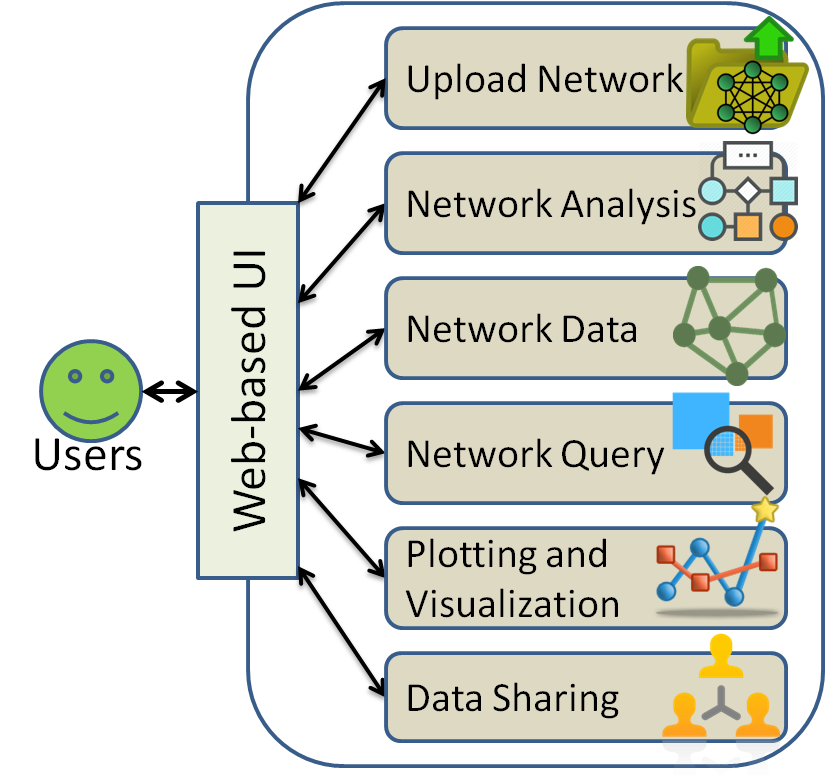
\includegraphics[trim = 0.0in 0.0in 0.0in 0.0in,scale=0.4]{user-features}
\caption{
Features of the NEMO system.
}   %   
\label{fig:user-features}
\end{figure}

\subsection{Features}

\begin{itemize}
\item Exposes the MARS network repository, with the ability to filter and search for networks.
\item Exposes MARS network query service. Users can interactively run queries against network data and download the query results.
\item Analysis of network data using MARS workflow service.
\item Generates publication-quality graphics while interactively explore the data.
\item Network visualization using gephi service.

\end{itemize}





\line(1,0){500}

\section{NEMO Setup}

\subsection{Installation}


Step to install NEMO:
Note: Wavemaker has been used and tested on windows 7. There is a version available for Mac. To use wavemaker, basic web development skills are required (e.g. html, css, javascript).
\begin{itemize}
\item Need first to install and start MARS services v2.0, please see MARS manual. NEMO is currently using three services Network Query Service (NQS), Network Search Service (NSS) and Network Workflow Service (NWS). 
\item NEMO v1 is developed using Wavemaker framework. Need to checkout/download the NEMO (.war and .zip files) from git repo. Git URL is https://ndsslgit.vbi.vt.edu/software-knowledge-discovery/kd-01.git
\item Start Wavemaker on local machine using desktop launcher tool. See Figure~\ref{fig:launcher}. Note: the server will start automatically. Once started, the default browser will open automatically with the wavemaker landing page.

\begin{figure}[H]
\centering
%\label{fig:ebola-kshell-not-effective}
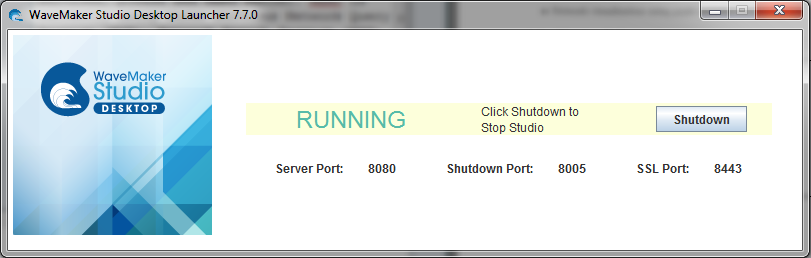
\includegraphics[trim = 0.0in 0.0in 0.0in 0.0in,scale=0.4]{launcher}
\caption{
Wavemaker desktop launcher
}   %   
\label{fig:launcher}
\end{figure}

\item Once Wavemaker framework started, use the import feature to load the .zip file into your working environment, and name the project NEMO.

\begin{figure}[H]
\centering
%\label{fig:ebola-kshell-not-effective}
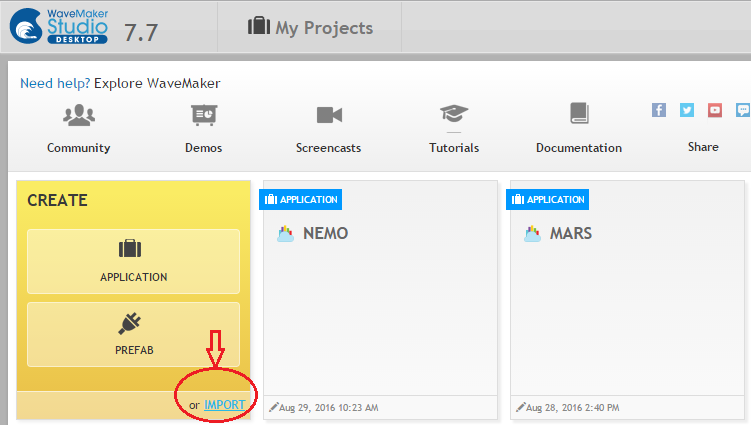
\includegraphics[trim = 0.0in 0.0in 0.0in 0.0in,scale=0.6]{import}
\caption{
Import project in Wavemaker.
}   %   
\label{fig:import}
\end{figure}

\end{itemize}

Steps to setup Netviewer:
Note: NEMO is using a network visualization web application (netviewer). Netviewer is a thin-layer using Gephi and GEXF viewer. 
\begin{itemize}
\item Convert the network .uel file to .csv format.
\item Import the .csv file to gephi. Note: gephi has to be installed on your local machine.
\item Use any visualization or layout algorithm of choice to generate a visualization of the network. Please see gephi manual for different functionality.
\item Once done, click $file->export->graph$ file and choose .gexf. Name the file exactly as the network name.
\item Place the .gexf file under the netviewer dirctory.


\end{itemize}
The app is currently deployed on edisondev VM at /apps/apache-tomcat-7.0.40/webapps/netviewer. The code for the app is available in the git repo at src/netviewer. To deploy netviewer just upload the folder netviewer to the required webapp dir on the VM. 

\line(1,0){500}

\section{Project Overview}
Note: the wavemaker reference manual is available at (http://www.wavemaker.com/learn/documentation-reference/ ). 

Wavemaker provides a set of different project views, see Figure~\ref{fig:workspace}. The \textbf{design view}, accessed by the button inside the green circle, allows users to design the web interface using a drag-and-drop approach. At any time users can switch to the \textbf{script view}, by clicking on the button inside the blue circle, to add event-handlers in javascript. Wavemaker is using angularjs which is a javascript library. To add an \textbf{event handler} to a control in the UI, use the button (inside the red circle) with hand-like caption. To edit an existing \textbf{control properties}, use the button (inside the black circle) with the palette-like caption.  
To integrate a \textbf{new service}, click on import (inside the brown circle) then click new web service. Follow the steps in the wizard to define the new service with its parameters. To update an existing service, click on services link (inside the orange circle) on the left-hand side. NEMO has multiple design views, to switch to another view click on the button \textbf{select view} inside the purple circle. Please read wavemaker manual for additional functionality.

\begin{figure}[H]
\centering
%\label{fig:ebola-kshell-not-effective}
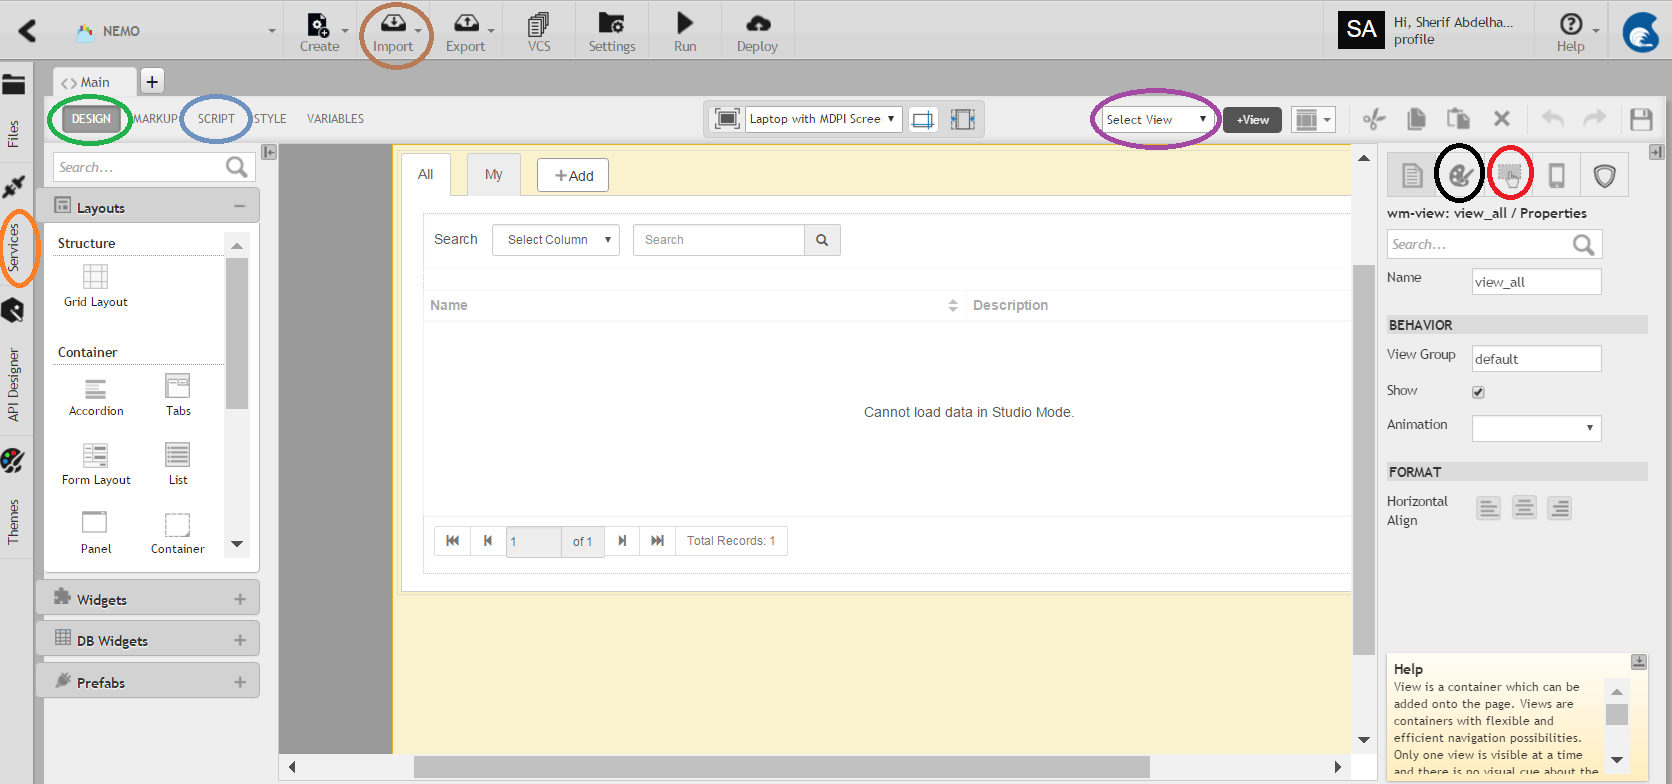
\includegraphics[trim = 0.0in 0.0in 0.0in 0.0in,scale=0.5]{workspace}
\caption{
Project workspace in Wavemaker. Each circle refer to different functionality.
}   %   
\label{fig:workspace}
\end{figure}

\line(1,0){500}
\section{NEMO deployment}
\begin{itemize}
\item Save the project by clicking on the save button on the top right. Note: it is preferable to save the project every time before deployment. 

\item Export the project in both .zip and .war formats.

\item Upload the .war file to your VM webApp Folder. For example, in edisondev VM the webApp directory is /apps/apache-tomcat-7.0.40/webapps. 
\end{itemize}

\line(1,0){500}

\section{Using Nemo as End User}

\subsection{User Authentication} 
When NEMO application is loaded, users are authenticated through username and password for login. Currently, there are two user roles (user and admin). Figure~\ref{fig:login-screen} shows NEMO sign in page.  

\begin{figure}[H]
\centering
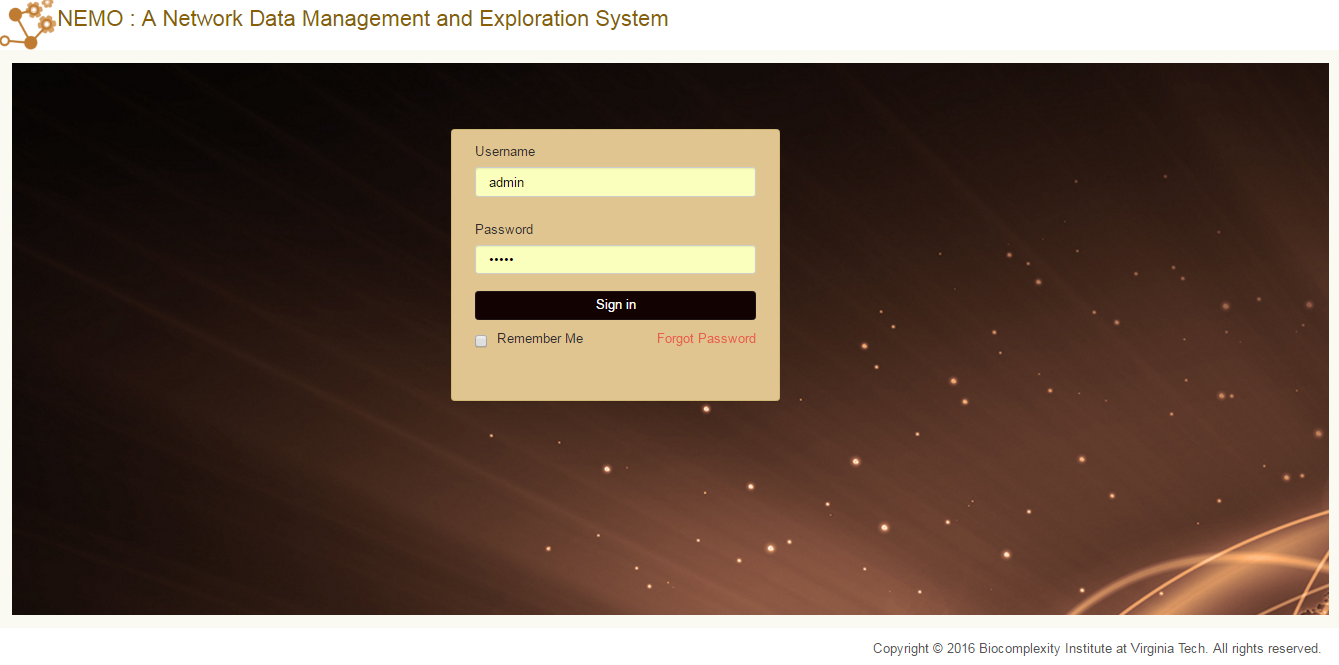
\includegraphics[trim = 0.0in 0.0in 0.0in 0.0in,scale=0.55]{login-screen}
\caption{
NEMO login page.
}   %   
\label{fig:login-screen}
\end{figure}

\subsection{Network Repository}
Once a user signed in, NEMO displays the network list view, see Figure~\ref{fig:network-list-screen}. There are two lists, a public list of networks added by current user and other users, where network is marked public. The other list contains networks owned by current user and might not necessarily be available for public. Users can search for a network by keyword(s) against a selected attribute (network name or description).

\begin{figure}[H]
\centering
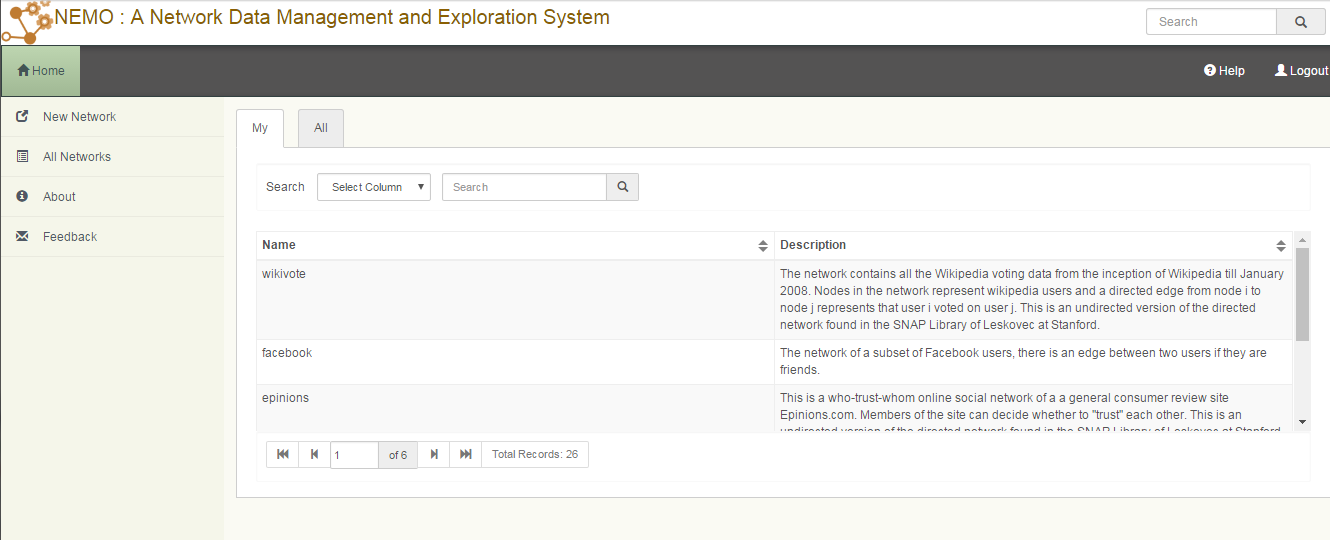
\includegraphics[trim = 0.0in 0.0in 0.0in 0.0in,scale=0.55]{network-list-screen}
\caption{
NEMO login page.
}   %   
\label{fig:network-list-screen}
\end{figure}


\subsection{Network Information}
By clicking on a network record in the network list, NEMO takes the user to another view that shows more detailed information including computer node and edge measures, see Figure. At any time users can proceed with further network visualization, analysis or return back to the network repository. 

\begin{figure}[H]
\centering
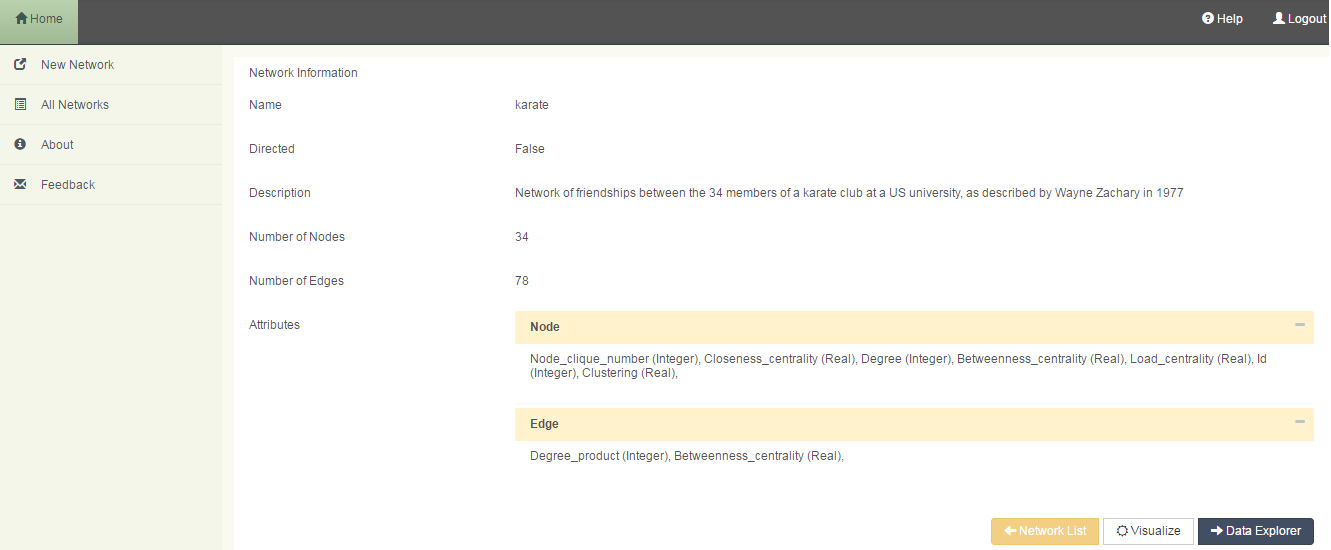
\includegraphics[trim = 0.0in 0.0in 0.0in 0.0in,scale=0.45]{network-info-screen2}
\caption{
Detailed information of a selected network Karate.
}   %   
\label{fig:network-info-screen2}
\end{figure}

\subsection{Network Visualization}
The visualization in Figure~\ref{fig:network-visualization3-screen} is generated with NEMO, using Gephi and a thin layer consisting of a Javascript GEXF
Viewer, available for download. Network visualization can be accessed through NEMO or directly through a supported separate URL. Visualizations can also be embedded into external websites. The visualization component resides on a separate machine from NEMO, which allows re-configuration or upgrading the visualization layer without affecting NEMO.
\begin{figure}[H]
\centering
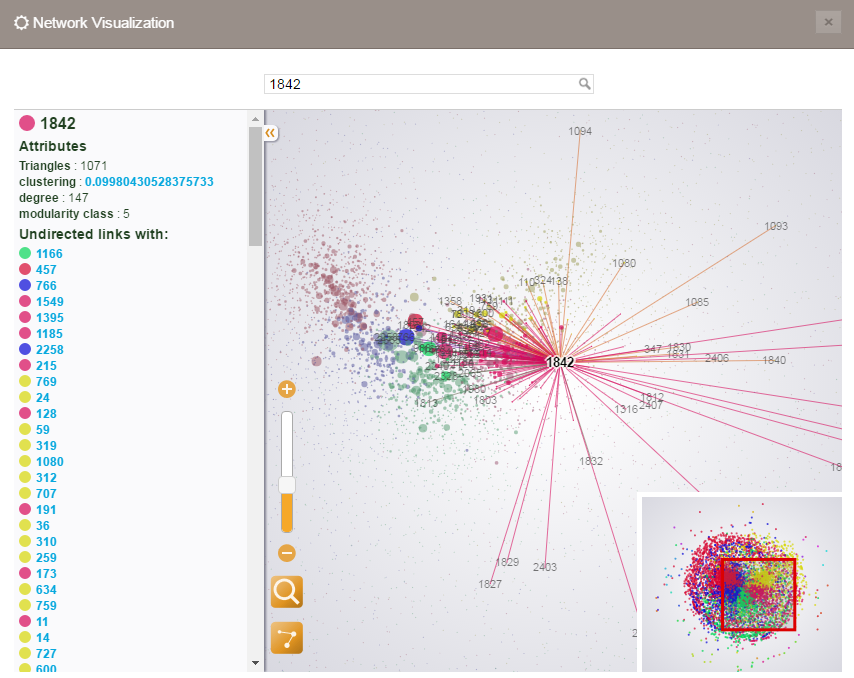
\includegraphics[trim = 0.0in 0.0in 0.0in 0.0in,scale=0.45]{network-visualization3-screen}
\caption{
Detailed information of a selected network Karate.
}   %   
\label{fig:network-visualization3-screen}
\end{figure}

\subsection{Data Explorer}

NEMO data explorer provides two ways for analyzing network data and reasoning about simulation results. The \textbf{query tab} allows the user to interact with MARS network query service. In addition to regular queries, user can run sampling queries for seed nodes/edges. Return data can be vertex IDs only, or IDs with all properties associated with
each vertex. Similarly for edge-based queries. This is useful for queries that produce large return sets; if all that is needed
are vertex (resp. edge) IDs, then much storage can be saved. Currently results can be copied to clipboard, but downloading the results is possible.

\begin{figure}[H]
\centering
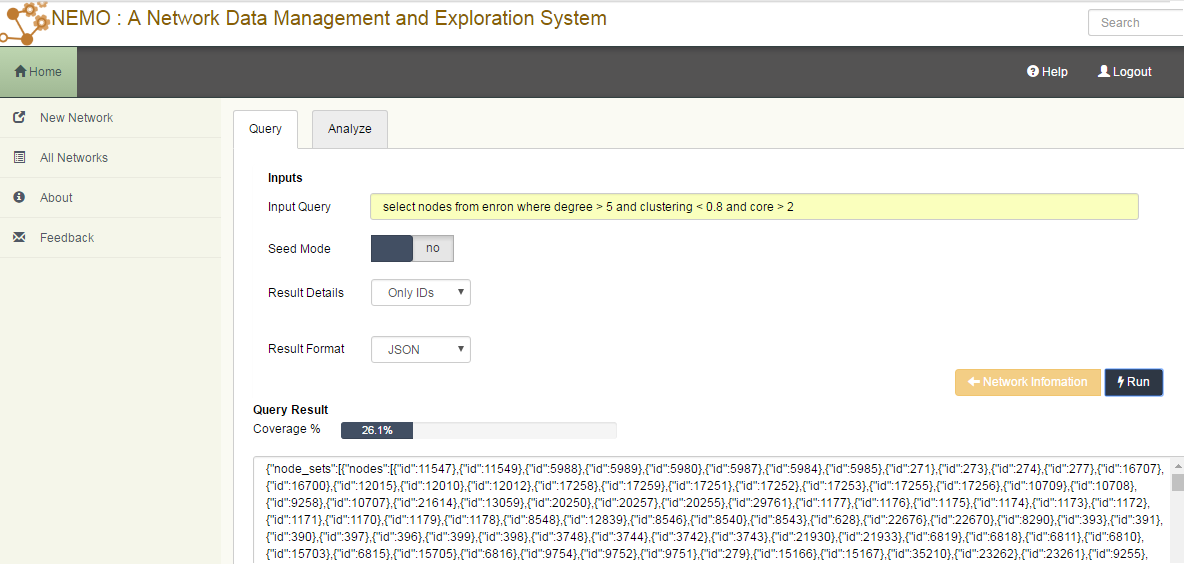
\includegraphics[trim = 0.0in 0.0in 0.0in 0.0in,scale=0.45]{network-query-screen-quality}
\caption{
NEMO screen for performing queries. The specified query returns all vertices that have degree > 5, clustering
coefficient < 0.8, and k-core of 3 or more. Result formats include JSON and XML. The particular
query returned 26.1% of network vertices.
}   %   
\label{fig:network-query-screen-quality}
\end{figure}

The \textbf{Analyze tab} provides a medium (workflow designer, see Figure~\ref{fig:network-wf-list-screen-new-5}) for users to construct workflows for network data analysis and plotting. 
\begin{figure}[H]
\centering
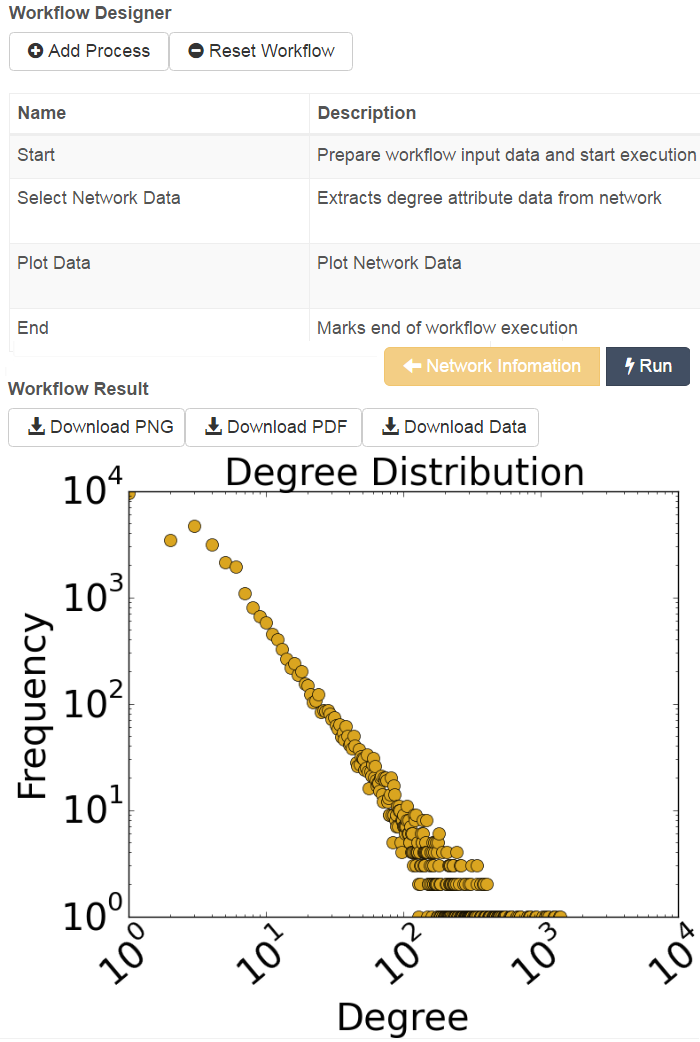
\includegraphics[trim = 0.0in 0.0in 0.0in 0.0in,scale=0.45]{network-wf-list-screen-new-5}
\caption{
NEMO workflow designer. User can add, edit or delete workflow processes in iterative manner. The final result can be numeric, text or plot. The generated plots are publication-quality and can be downloaded  in either pdf or png formats. Users can even download the plot raw data, if they want to use their own plotting tool.
}   %   
\label{fig:network-wf-list-screen-new-5}
\end{figure}
 
 \subsection{Examples of Plots can be generated by NEMO}
 
 \begin{figure}[H]
    \centering
    \begin{subfigure}[b]{0.3\textwidth}
        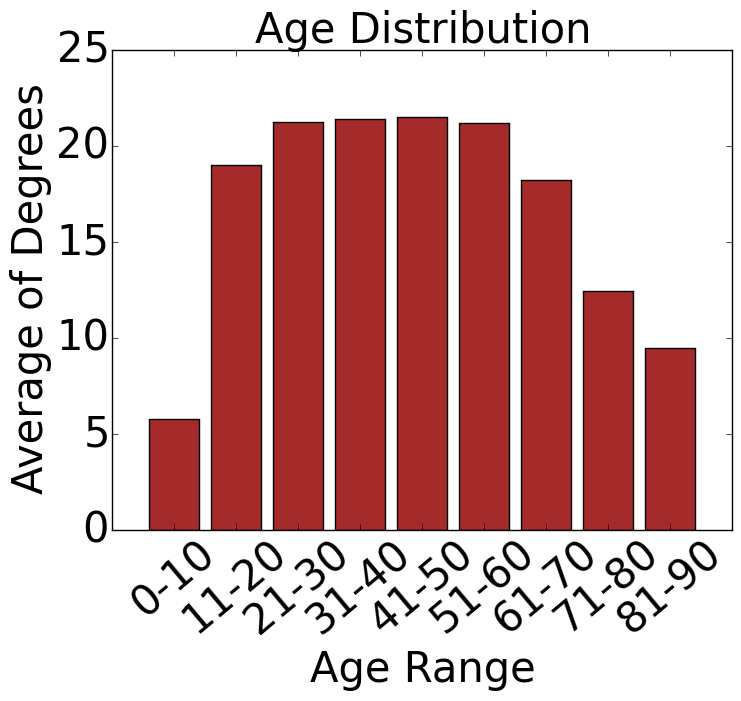
\includegraphics[width=\textwidth]{147}
        \caption{Average degree of a
person in each age bin.}
        \label{fig:147}
    \end{subfigure}
    ~ %add desired spacing between images, e. g. ~, \quad, \qquad, \hfill etc. 
      %(or a blank line to force the subfigure onto a new line)
    \begin{subfigure}[b]{0.3\textwidth}
        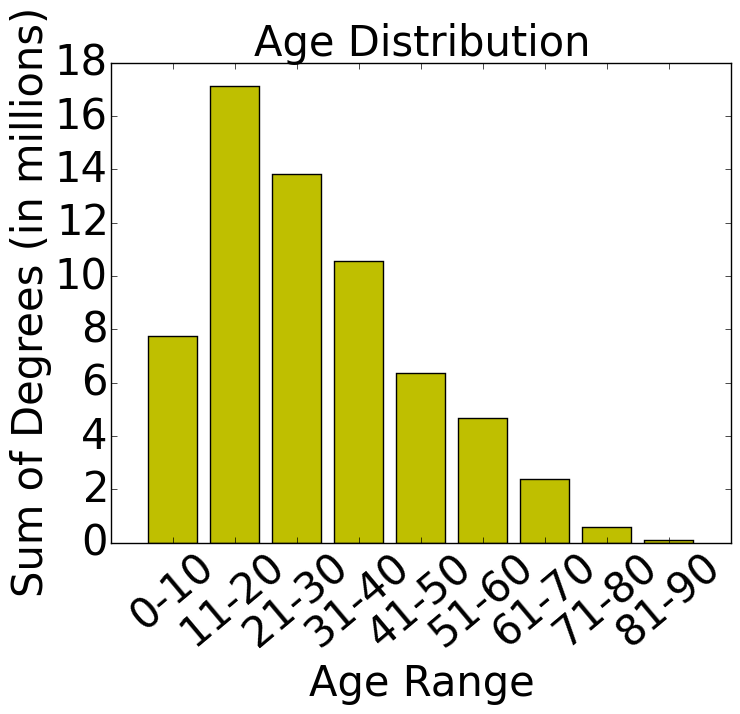
\includegraphics[width=\textwidth]{137}
        \caption{Total number of edges
formed by people in each age bin.}
        \label{fig:137}
    \end{subfigure}
    ~ %add desired spacing between images, e. g. ~, \quad, \qquad, \hfill etc. 
    %(or a blank line to force the subfigure onto a new line)
      \begin{subfigure}[b]{0.3\textwidth}
        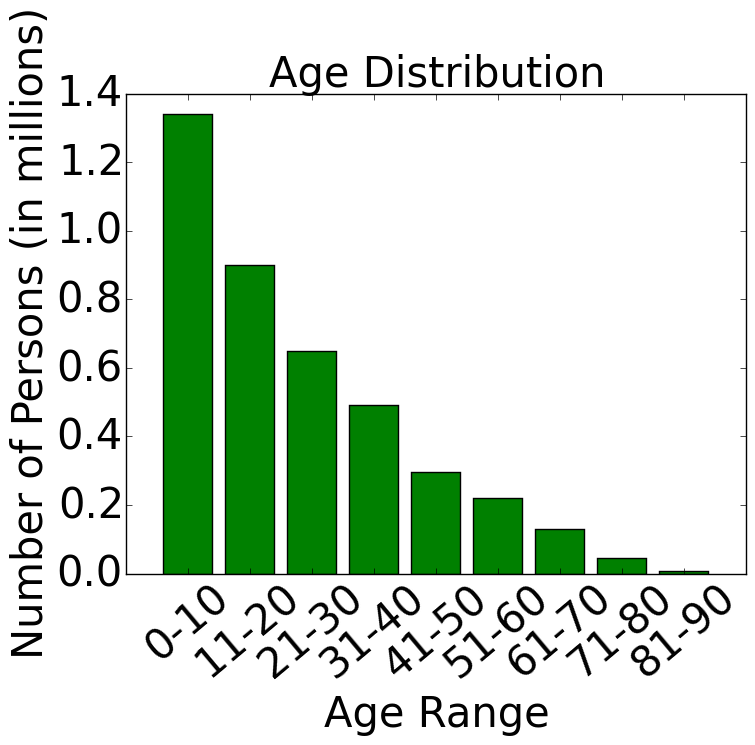
\includegraphics[width=\textwidth]{144}
        \caption{The number of people in each age range}
        \label{fig:144}
    \end{subfigure}
     \\
     \begin{subfigure}[b]{0.3\textwidth}
        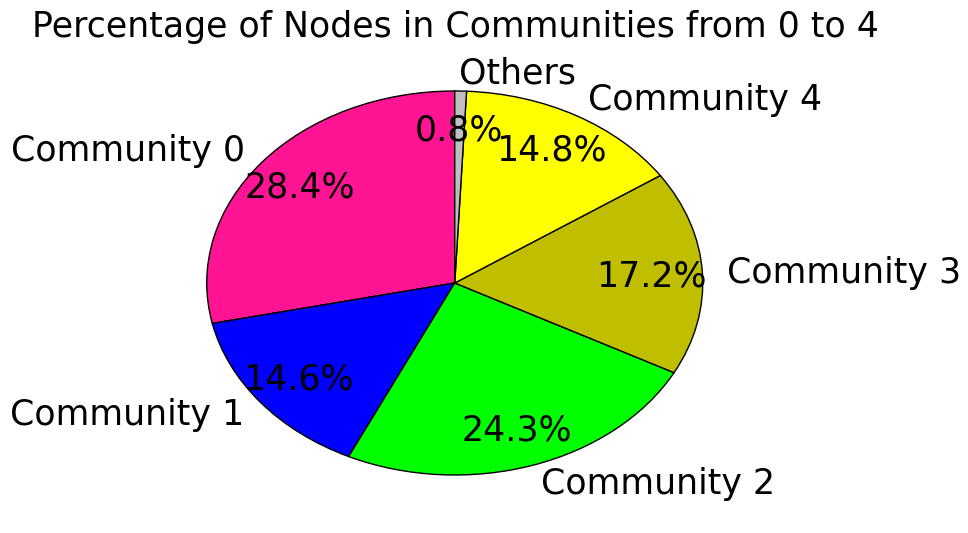
\includegraphics[width=\textwidth]{183}
        \caption{Fraction of vertices in each of the five largest communities
for a Wikivote network with 7115 vertices.}
        \label{fig:183}
    \end{subfigure}
    ~ 
     \begin{subfigure}[b]{0.3\textwidth}
        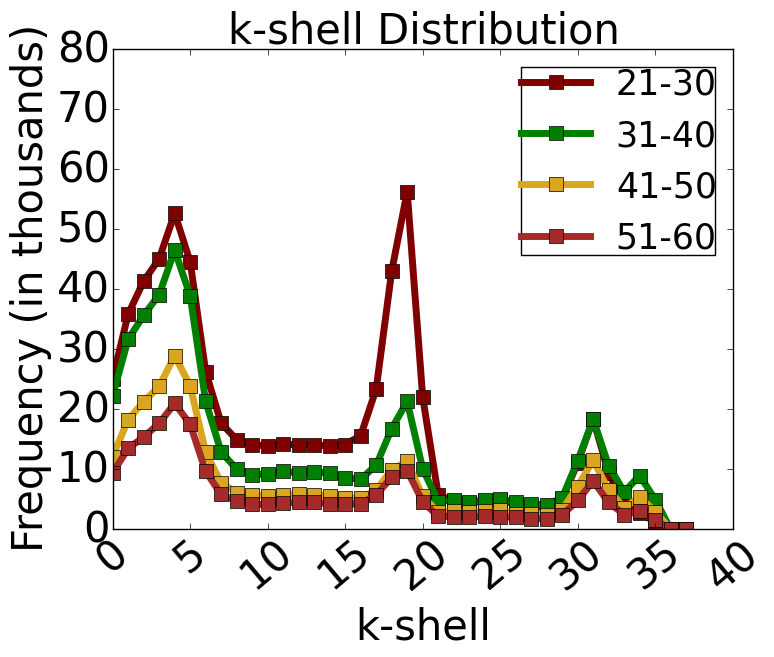
\includegraphics[width=\textwidth]{k-shell-1}
        \caption{The number of people in each age range, where the
ranges are 10-year increments.}
        \label{fig:k-shell-1}
    \end{subfigure}
    ~ 
     \begin{subfigure}[b]{0.3\textwidth}
        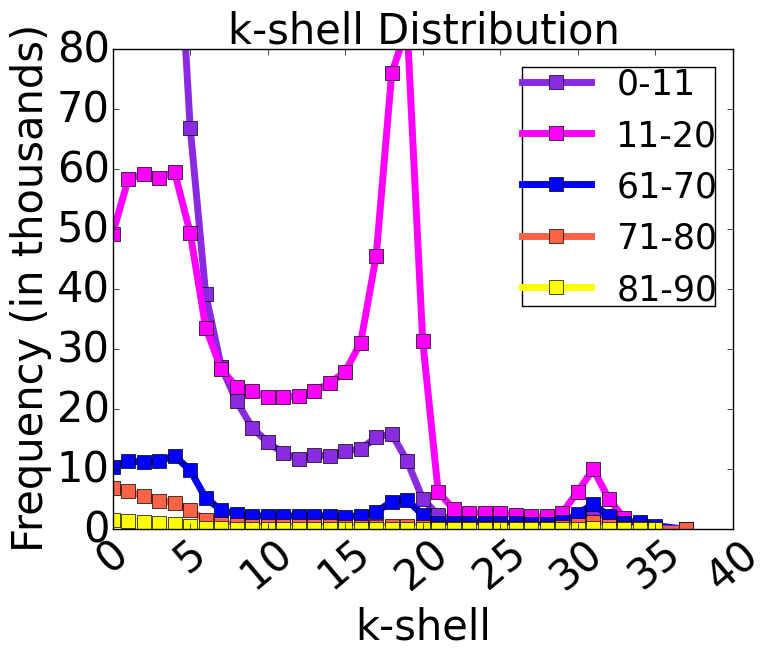
\includegraphics[width=\textwidth]{k-shell-2}
        \caption{The number of people in each age range, where the
ranges are 10-year increments.}
        \label{fig:k-shell-2}
    \end{subfigure}
    \\
    \begin{subfigure}[b]{0.3\textwidth}
        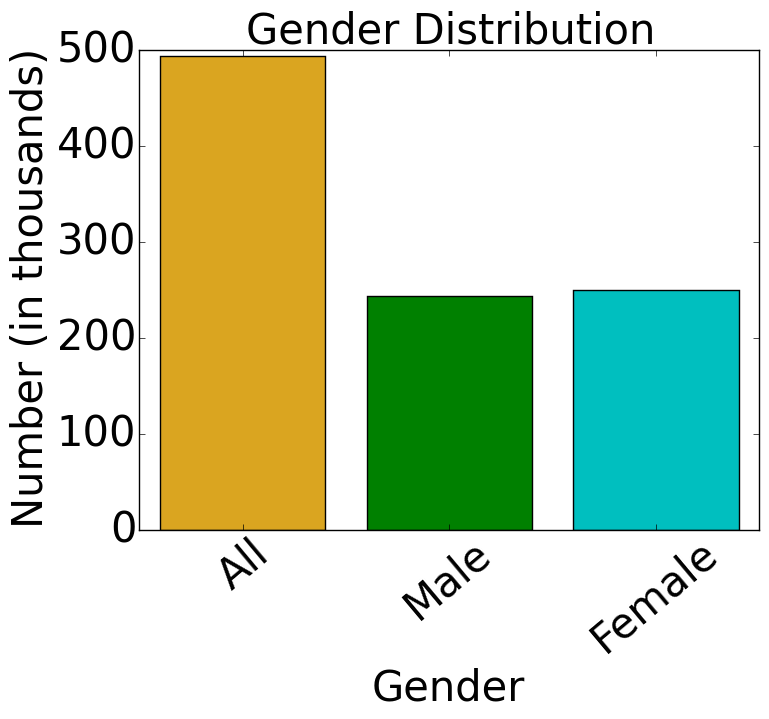
\includegraphics[width=\textwidth]{ebola-2}
        \caption{The number of people in each age range, where the
ranges are 10-year increments.}
        \label{fig:ebola-2}
    \end{subfigure}
    ~
    \begin{subfigure}[b]{0.3\textwidth}
        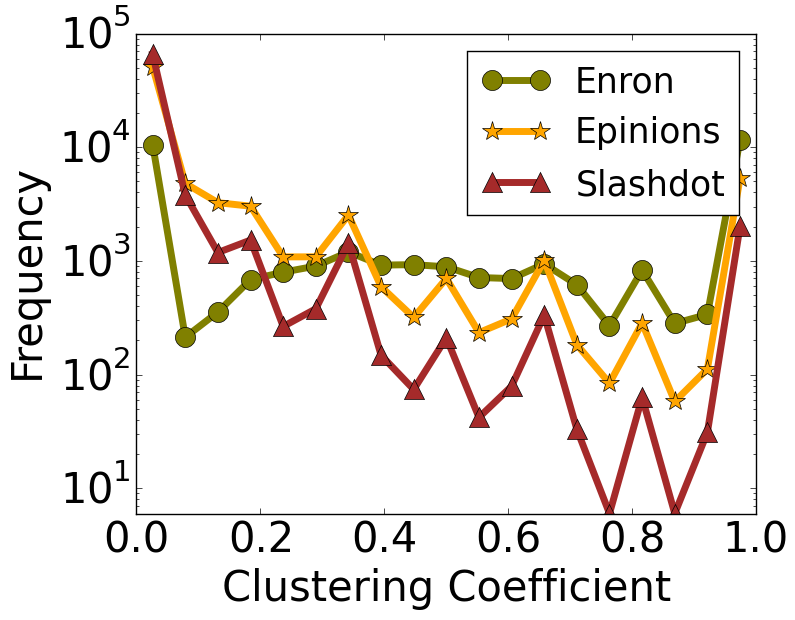
\includegraphics[width=\textwidth]{combined-clustering2}
        \caption{The number of people in each age range, where the
ranges are 10-year increments.}
        \label{fig:combined-clustering2}
    \end{subfigure}
    ~
    \begin{subfigure}[b]{0.3\textwidth}
        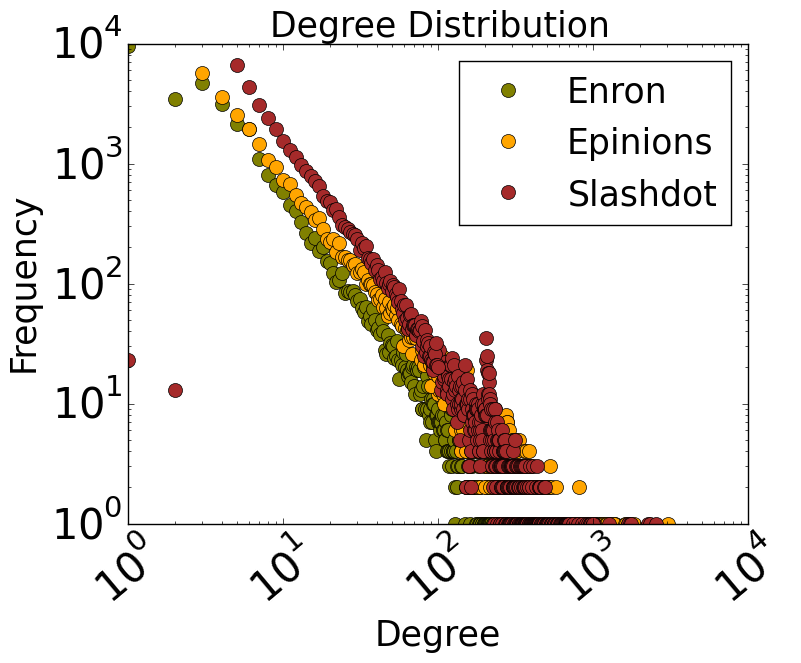
\includegraphics[width=\textwidth]{degree-combined}
        \caption{The number of people in each age range, where the
ranges are 10-year increments.}
        \label{fig:degree-combined}
    \end{subfigure}
    \caption{Different plots generated by NEMO workflows}\label{fig:nemo-plots}
\end{figure}



%
% ---- Bibliography ----
%

%\bibliographystyle{plain}
%\bibliography{refs-mnf-files}




\end{document}
